\section{Lattices and reciprocal space}\label{sec:3.1}

A kilogram of silicon holds $2.1\times10^{25}$ atoms, and every one of them sits at a point of a lattice that repeats the same pair of atoms in every direction. The repetition has two consequences that every later rate uses: a crystal conserves momentum only up to a reciprocal-lattice vector, the working definition of \cref{sec:1.3}, and the momenta it can tell apart fill a single cell of reciprocal space, the Brillouin zone. We construct both for the diamond structure of silicon, count the states in the zone, and measure the momentum transfers of \cref{sec:1.3} against the size of the zone. The material is standard, and we follow Refs.~\cite[Chaps.~4--6 and 8]{ashcroft1976solid} and \cite[Chaps.~1--2]{kittel2005introduction}.

Throughout \cref{chap:3,chap:4} the nuclei sit at fixed equilibrium positions: we work with a \emph{static lattice}. The approximation rests on the mass ratio. A silicon nucleus is $M/m_e = \num{5.1e4}$ times heavier than an electron, and the electrons rearrange long before the nuclei have moved appreciably. \Cref{sec:5.1} makes this precise with the Born--Oppenheimer expansion. What the static lattice leaves out are the vibrations themselves, phonons, and their coupling to the electrons, which \cref{chap:5,chap:6} add back.

\subsection{Bravais lattice and basis}

A \emph{Bravais lattice} is the set of points
\begin{equation}
  \vect{R} = n_1\vect{a}_1 + n_2\vect{a}_2 + n_3\vect{a}_3, \qquad n_i \in \mathbb{Z},
  \label{eq:3.1-R}
\end{equation}
generated by three linearly independent \emph{primitive vectors} $\vect{a}_i$. Every lattice vector $\vect{R}$ maps the lattice onto itself. The parallelepiped spanned by the $\vect{a}_i$ is a primitive cell: its translations by all $\vect{R}$ fill space without overlap, and it contains one lattice point. Its volume,
\begin{equation}
  \Omega = \vect{a}_1\cdot(\vect{a}_2\times\vect{a}_3),
  \label{eq:3.1-Omega}
\end{equation}
is the \emph{cell volume}, the only meaning of a bare $\Omega$ in this book (a solid angle always carries a subscript, as in $\dd\Omega_q$). The choice of primitive vectors is not unique, but every primitive cell has the same volume, since each holds one lattice point.

A crystal places a group of atoms, the \emph{basis}, at every lattice point. We label the atoms of the basis by $\kappa = 1, \dots, n_{\mathrm{at}}$ and their positions within the cell by $\vect{\tau}_\kappa$, so that the nuclei sit at
\begin{equation}
  \vect{X}_{\vect{R}\kappa} = \vect{R} + \vect{\tau}_\kappa .
  \label{eq:3.1-X}
\end{equation}
This is the $\kappa$ that labels $Z_\kappa$ and $n_\kappa(\vect{k})$ in \cref{sec:2.3}; two sites of one element still carry different $\kappa$.

Silicon has the \emph{diamond structure} drawn in \cref{fig:3-diamond}. Its Bravais lattice is face-centered cubic (fcc): the corners and face centers of a cube of side $a$, the \emph{lattice constant}. A symmetric choice of primitive vectors joins a corner to the three nearest face centers,
\begin{equation}
  \vect{a}_1 = \frac{a}{2}(0,1,1), \qquad \vect{a}_2 = \frac{a}{2}(1,0,1), \qquad \vect{a}_3 = \frac{a}{2}(1,1,0),
  \label{eq:3.1-fcc}
\end{equation}
and \cref{eq:3.1-Omega} yields $\Omega = a^3/4$: the cube contains four lattice points. The basis consists of two silicon atoms,
\begin{equation}
  \vect{\tau}_1 = 0, \qquad \vect{\tau}_2 = \frac{a}{4}(1,1,1),
  \label{eq:3.1-basis}
\end{equation}
displaced along the cube diagonal by a quarter of its length. Each atom then has four nearest neighbors at the corners of a regular tetrahedron, at the distance $\sqrt3\,a/4$ and with bond angles of \ang{109.47}. These are the four covalent bonds of a silicon atom, one for each valence electron, and \cref{sec:3.2} returns to the $sp^3$ orbitals that form them. Note that the diamond structure is not a Bravais lattice: the environment of an atom at $\vect{\tau}_2$ is that of an atom at $\vect{\tau}_1$ inverted through the bond center, and no lattice vector maps one onto the other.

\begin{figure}[tbp]
  \centering
  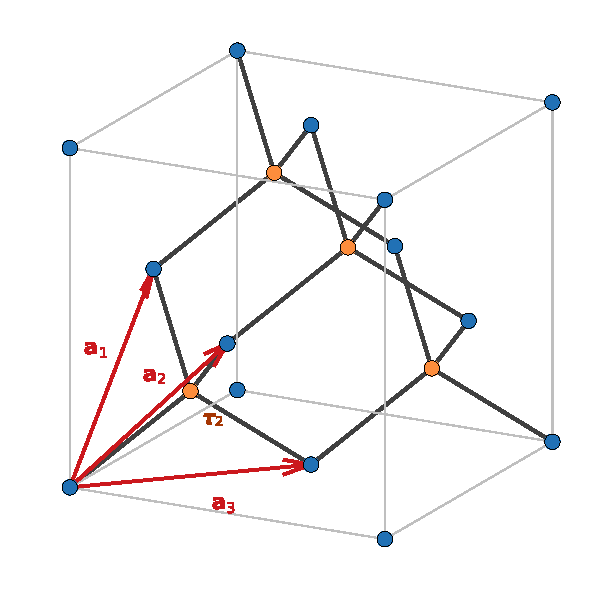
\includegraphics[width=0.55\linewidth]{figures/ch03/fig3_1.pdf}
  \caption{The diamond structure, drawn in a cube of side $a$, the lattice constant. Blue: the face-centered cubic lattice of sites $\vect{R}$ (cube corners and face centers). Orange: the second atom of the basis, at $\vect{R} + \vect{\tau}_2$ with $\vect{\tau}_2 = (a/4)(1,1,1)$; the four inside the cube are shown. Dark lines join nearest neighbors, at a distance $\sqrt3\,a/4$, \SI{2.352}{\angstrom} in silicon ($a = \SI{5.431}{\angstrom}$); each atom is bonded to four others at the corners of a regular tetrahedron. Red arrows: the primitive vectors $\vect{a}_1 = (a/2)(0,1,1)$, $\vect{a}_2 = (a/2)(1,0,1)$, $\vect{a}_3 = (a/2)(1,1,0)$, which span a primitive cell of volume $a^3/4$ containing two atoms. In the zincblende structure (GaAs) the blue and orange sites hold different elements.}
  \label{fig:3-diamond}
\end{figure}

The lattice constant of silicon is $a = \SI{5.431}{\angstrom}$~\cite[lattice parameter of silicon]{mohr2025codata}, or $\num{2.752e-3}\,\mathrm{eV}^{-1}$ in natural units. The cell volume is $\Omega = \SI{40.05}{\angstrom^3}$, the nearest-neighbor distance is \SI{2.352}{\angstrom}, and the cube of side $a$ holds eight atoms. These numbers fix the densities used in the earlier chapters. The atomic density is $8/a^3 = \SI{4.99e22}{cm^{-3}}$, which with the atomic weight 28.0855 yields the mass density \SI{2.33}{g.cm^{-3}} of \cref{sec:1.2}. With four valence electrons per atom, the valence density $32/a^3 = \SI{2.00e23}{cm^{-3}}$ is the one used for the free electron gas of \cref{sec:2.5}. Germanium has the same structure with a lattice constant a few percent larger. Gallium arsenide has the \emph{zincblende structure}, the same lattice and the same $\vect{\tau}_\kappa$, but with gallium at $\vect{\tau}_1$ and arsenic at $\vect{\tau}_2$~\cite[Chap.~4]{ashcroft1976solid}. Since the two sites now differ, the inversion that exchanged them in silicon is no longer a symmetry. As a result GaAs is polar, a property that matters for its phonons (\cref{sec:5.5}). \Cref{sec:3.3} gives the band structures of all three materials.

A first-principles calculation, in density-functional theory (\cref{sec:3.4}), either takes $a$ from experiment or finds it by minimizing the computed total energy of the crystal with respect to $a$ (\cref{app:E.1}). For silicon in the local-density approximation the minimum lies at \SI{5.401}{\angstrom}, \SI{0.5}{\percent} below the measured value~\cite[Sect.~10.2]{ponce2016epw}. A rate is usually computed at the measured $a$. Since band energies depend on $a$, the choice shifts the computed gap, one of the reasons why computed and measured thresholds differ (\cref{sec:3.4}).

\subsection{The reciprocal lattice}

A plane wave $\ee^{\ii\vect{G}\cdot\vect{r}}$ that takes the same value at every lattice point, $\ee^{\ii\vect{G}\cdot\vect{R}} = 1$ for all $\vect{R}$, is the building block of every function with the periodicity of the lattice. The wavevectors $\vect{G}$ with this property are the \emph{reciprocal-lattice vectors}. By \cref{eq:3.1-R} the condition holds for all $\vect{R}$ if and only if $\vect{G}\cdot\vect{a}_i$ is a multiple of $2\pi$ for each $i$. We therefore look for vectors $\vect{b}_j$ with
\begin{equation}
  \vect{a}_i\cdot\vect{b}_j = 2\pi\delta_{ij} .
  \label{eq:3.1-dual}
\end{equation}
They are
\begin{equation}
  \vect{b}_1 = \frac{2\pi}{\Omega}\,\vect{a}_2\times\vect{a}_3, \qquad
  \vect{b}_2 = \frac{2\pi}{\Omega}\,\vect{a}_3\times\vect{a}_1, \qquad
  \vect{b}_3 = \frac{2\pi}{\Omega}\,\vect{a}_1\times\vect{a}_2 .
  \label{eq:3.1-b}
\end{equation}
To check \cref{eq:3.1-dual}, note that $\vect{a}_1\cdot\vect{b}_1 = 2\pi\,\vect{a}_1\cdot(\vect{a}_2\times\vect{a}_3)/\Omega = 2\pi$ by \cref{eq:3.1-Omega}, while $\vect{a}_2\cdot\vect{b}_1$ and $\vect{a}_3\cdot\vect{b}_1$ vanish because a triple product with a repeated vector is zero; the other components follow by cyclic permutation. Since the $\vect{b}_j$ are linearly independent, any wavevector can be written as $\vect{G} = \sum_jm_j\vect{b}_j$ with real $m_j$, and then $\vect{G}\cdot\vect{a}_i = 2\pi m_i$. The condition $\ee^{\ii\vect{G}\cdot\vect{R}} = 1$ thus requires integer $m_i$, and the reciprocal-lattice vectors form a Bravais lattice of their own,
\begin{equation}
  \vect{G} = m_1\vect{b}_1 + m_2\vect{b}_2 + m_3\vect{b}_3, \qquad m_i \in \mathbb{Z},
  \label{eq:3.1-G}
\end{equation}
with primitive vectors $\vect{b}_i$. In the book's convention (\cref{app:A.3}), a function with the periodicity of the lattice is a sum $f(\vect{r}) = \sum_{\vect{G}}f_{\vect{G}}\,\ee^{-\ii\vect{G}\cdot\vect{r}}$ over these vectors, with $f_{\vect{G}} = \Omega^{-1}\int_\Omega\dd^3r\,\ee^{\ii\vect{G}\cdot\vect{r}}f(\vect{r})$ (\cref{eq:A.3-periodic}). The plane wave $\ee^{\ii\vect{G}\cdot\vect{r}}$ is constant on planes perpendicular to $\vect{G}$, and for the shortest $\vect{G}$ in a given direction its wavelength $2\pi/|\vect{G}|$ is the spacing of the lattice planes perpendicular to it.

The volume of the cell spanned by the $\vect{b}_i$ follows from \cref{eq:3.1-b}. With the identity $(\vect{u}\times\vect{v})\times(\vect{u}\times\vect{w}) = \vect{u}\,[\vect{u}\cdot(\vect{v}\times\vect{w})]$ for $\vect{u} = \vect{a}_1$,
\begin{equation*}
  \vect{b}_2\times\vect{b}_3 = \frac{(2\pi)^2}{\Omega^2}\,(\vect{a}_3\times\vect{a}_1)\times(\vect{a}_1\times\vect{a}_2) = \frac{(2\pi)^2}{\Omega^2}\,\vect{a}_1\,[\vect{a}_1\cdot(\vect{a}_2\times\vect{a}_3)] = \frac{(2\pi)^2}{\Omega}\,\vect{a}_1 ,
\end{equation*}
where the sign of the first cross product was reversed to bring $\vect{a}_1$ to the front of both factors, and the sign of the second triple product with it. Then \cref{eq:3.1-dual} gives
\begin{equation}
  \vect{b}_1\cdot(\vect{b}_2\times\vect{b}_3) = \frac{(2\pi)^3}{\Omega} .
  \label{eq:3.1-BZvol}
\end{equation}
A small cell in real space is a large one in reciprocal space, as the Fourier transform requires.

For the fcc vectors of \cref{eq:3.1-fcc}, \cref{eq:3.1-b} yields
\begin{equation}
  \vect{b}_1 = \frac{2\pi}{a}(-1,1,1), \qquad \vect{b}_2 = \frac{2\pi}{a}(1,-1,1), \qquad \vect{b}_3 = \frac{2\pi}{a}(1,1,-1),
  \label{eq:3.1-bfcc}
\end{equation}
as we can confirm directly from \cref{eq:3.1-dual}: for instance, $\vect{a}_1\cdot\vect{b}_1 = \pi(0 + 1 + 1) = 2\pi$ and $\vect{a}_2\cdot\vect{b}_1 = \pi(-1 + 0 + 1) = 0$. These are the primitive vectors of a body-centered cubic lattice. Writing $\vect{G} = (2\pi/a)(h,k,l)$, \cref{eq:3.1-G} reads $h = -m_1 + m_2 + m_3$ and its cyclic permutations, so that $h + k = 2m_3$, $k + l = 2m_1$ and $l + h = 2m_2$. The reciprocal-lattice vectors of the fcc lattice are the vectors $(2\pi/a)(h,k,l)$ with integers $h, k, l$ that are all even or all odd, and every such triple occurs. The integers are the Miller indices of the lattice planes perpendicular to $\vect{G}$, and we write $\vect{G}_{hkl}$. The shortest nonzero vectors are the eight $\vect{G}_{111}$ along the cube diagonals, with $|\vect{G}_{111}| = \sqrt3\,2\pi/a$, followed by the six $\vect{G}_{200}$ along the cube axes, with $|\vect{G}_{200}| = 2\cdot2\pi/a$. In silicon $2\pi/a = \SI{2.28}{keV} = \SI{1.16}{\angstrom^{-1}}$, $|\vect{G}_{111}| = \SI{3.95}{keV}$ and $|\vect{G}_{200}| = \SI{4.57}{keV}$, the scales already met in \cref{sec:1.3,sec:2.4}.

\subsection{The Brillouin zone}

Two wavevectors that differ by a reciprocal-lattice vector give the same phase at every lattice point, $\ee^{\ii(\vect{k} + \vect{G})\cdot\vect{R}} = \ee^{\ii\vect{k}\cdot\vect{R}}$, and a lattice cannot tell them apart. The wavevectors that a crystal can distinguish fill one primitive cell of the reciprocal lattice. The conventional choice of cell is the \emph{first Brillouin zone}, the set of points closer to the origin than to any other reciprocal-lattice vector (\cref{sec:1.3}). The same construction around a point of the direct lattice, the points closer to it than to any other lattice point, is the \emph{Wigner--Seitz cell}, so the first Brillouin zone is the Wigner--Seitz cell of the reciprocal lattice. Its boundary is made of pieces of the planes $\vect{k}\cdot\vect{G} = |\vect{G}|^2/2$ that bisect the vectors $\vect{G}$, and a point on the boundary is equidistant from the origin and from at least one $\vect{G}$. The zone has the full point symmetry of the lattice, which is why it is preferred to the parallelepiped spanned by the $\vect{b}_i$. Both cells tile reciprocal space under translations by $\vect{G}$, and the zone has the volume of \cref{eq:3.1-BZvol}, $(2\pi)^3/\Omega$. For fcc it is $4(2\pi/a)^3$.

\begin{figure}[tbp]
  \centering
  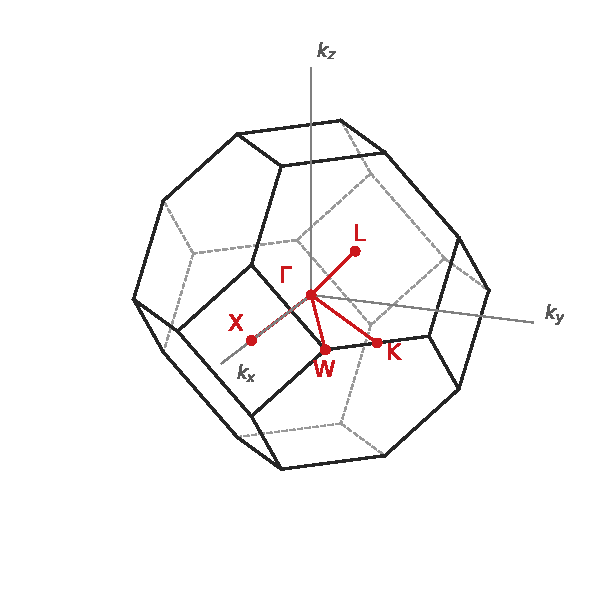
\includegraphics[width=0.52\linewidth]{figures/ch03/fig3_2.pdf}
  \caption{The first Brillouin zone of the face-centered cubic lattice, a truncated octahedron with eight hexagonal faces, which bisect the vectors $\vect{G}_{111} = (2\pi/a)(\pm1,\pm1,\pm1)$, and six square faces, which bisect $\vect{G}_{200} = (2\pi/a)(\pm2,0,0)$ and its permutations. Dashed edges are hidden. The high-symmetry points, in units of $2\pi/a$, are $\mathrm{\Gamma} = (0,0,0)$, $\mathrm{X} = (1,0,0)$, $\mathrm{L} = (\tfrac12,\tfrac12,\tfrac12)$, $\mathrm{K} = (\tfrac34,\tfrac34,0)$ and $\mathrm{W} = (1,\tfrac12,0)$; their distances from $\mathrm{\Gamma}$ are 1, 0.866, 1.061 and 1.118, or 2.28, 1.98, 2.42 and \SI{2.55}{keV} for silicon ($a = \SI{5.431}{\angstrom}$). The zone volume is $4(2\pi/a)^3 = (2\pi)^3/\Omega$.}
  \label{fig:3-bz}
\end{figure}

For the fcc lattice the zone is the truncated octahedron of \cref{fig:3-bz}. The planes that bisect the eight $\vect{G}_{111}$ cut out an octahedron, $|k_x| + |k_y| + |k_z| \le \tfrac32(2\pi/a)$, and the planes that bisect the six $\vect{G}_{200}$, $|k_x|, |k_y|, |k_z| \le 2\pi/a$, cut off its six corners; no longer $\vect{G}$ contributes a face. Points of high symmetry carry standard labels. The zone center is $\mathrm{\Gamma}$. The centers of the square faces are the six $\mathrm{X} = (2\pi/a)(1,0,0)$, at a distance $2\pi/a$, and the centers of the hexagonal faces are the eight $\mathrm{L} = (2\pi/a)(\tfrac12,\tfrac12,\tfrac12)$, at $\tfrac{\sqrt3}{2}\,2\pi/a$, the closest boundary points to $\mathrm{\Gamma}$. The midpoints of the edges shared by two hexagons are the points $\mathrm{K} = (2\pi/a)(\tfrac34,\tfrac34,0)$, and the corners are the points $\mathrm{W} = (2\pi/a)(1,\tfrac12,0)$, at $\tfrac{\sqrt5}{2}\,2\pi/a$, the farthest. The zone points are set upright, $\mathrm{\Gamma}$, $\mathrm{X}$, $\mathrm{L}$, $\mathrm{K}$, $\mathrm{W}$, to keep them apart from the italic rates $\varGamma$ of \cref{chap:2} and the loss function $L$ of \cref{sec:4.4}. A band structure is plotted along straight lines between these points, such as $\mathrm{L}$--$\mathrm{\Gamma}$--$\mathrm{X}$, and the band extrema of silicon, germanium and GaAs lie on them (\cref{sec:3.3}).

For silicon the zone is about \SI{2.3}{keV} in radius: every momentum shorter than $|\mathrm{\Gamma L}| = \SI{1.98}{keV}$ lies inside it, and every momentum longer than $|\mathrm{\Gamma W}| = \SI{2.55}{keV}$ lies outside. A sphere of the same volume has the radius $(3/\pi)^{1/3}\,2\pi/a = 0.985\,(2\pi/a) = \SI{2.25}{keV}$.

\subsection{Crystal momentum and the lattice sum}

With the nuclei clamped at the sites of \cref{eq:3.1-X}, the Hamiltonian of the electrons, \cref{eq:2.3-HC} without the nuclear kinetic energy, is unchanged when all electrons are moved by the same lattice vector $\vect{R}$, but not by an arbitrary vector. Let $T_{\vect{R}}$ be the operator that does this, $(T_{\vect{R}}\Psi)(\vect{r}_1, \dots, \vect{r}_{N_e}) = \Psi(\vect{r}_1 + \vect{R}, \dots, \vect{r}_{N_e} + \vect{R})$ for a wavefunction of $N_e$ electrons (spins are not moved). It is unitary, it commutes with the Hamiltonian, and translations compose, $T_{\vect{R}}T_{\vect{R}'} = T_{\vect{R} + \vect{R}'}$. As a result, the eigenstates of the Hamiltonian can be chosen as eigenstates of all $T_{\vect{R}}$ at once, with eigenvalues $c(\vect{R})$ that are phases and obey $c(\vect{R} + \vect{R}') = c(\vect{R})c(\vect{R}')$. Writing $c(\vect{a}_i) = \ee^{2\pi\ii x_i}$ with real $x_i$, the composition rule requires $c(\vect{R}) = \ee^{2\pi\ii\sum_in_ix_i}$, and with \cref{eq:3.1-dual} this is
\begin{equation}
  T_{\vect{R}}\Psi = \ee^{\ii\vect{k}\cdot\vect{R}}\,\Psi, \qquad \vect{k} = \sum_ix_i\vect{b}_i .
  \label{eq:3.1-crystalmomentum}
\end{equation}
The wavevector $\vect{k}$ is the \emph{crystal momentum} of the state. It is defined only up to a reciprocal-lattice vector, since $\vect{k}$ and $\vect{k} + \vect{G}$ give the same eigenvalues, and we take it in the first Brillouin zone. This makes precise the working definition of \cref{sec:1.3}. For a free particle every translation is a symmetry, and $\vect{k}$ is the momentum; in a crystal just the lattice translations survive, and momentum is conserved modulo $\vect{G}$, as \cref{sec:2.3} found from the Coulomb Hamiltonian. The literature also writes ``quasi-momentum''; the two terms mean the same. For a single electron, \cref{eq:3.1-crystalmomentum} becomes Bloch's theorem, which \cref{sec:3.2} derives together with the form of the states.

A finite crystal needs boundary conditions, and the \emph{Born--von Karman} conditions are the periodic ones of the box of \cref{sec:2.1}, adapted to the lattice. The crystal is a block of $N = N_1N_2N_3$ cells, the vectors $\vect{R} = \sum_in_i\vect{a}_i$ with $0 \le n_i < N_i$, and a translation by $N_i\vect{a}_i$ acts as the identity. Its volume is
\begin{equation}
  \Vol = N\Omega ,
  \label{eq:3.1-V}
\end{equation}
the normalization volume of \cref{sec:2.1}. The condition $c(N_i\vect{a}_i) = \ee^{\ii N_i\vect{k}\cdot\vect{a}_i} = 1$ restricts the crystal momenta to
\begin{equation}
  \vect{k} = \sum_i\frac{m_i}{N_i}\,\vect{b}_i, \qquad m_i \in \mathbb{Z} .
  \label{eq:3.1-kgrid}
\end{equation}
Adding $N_i$ to $m_i$ adds $\vect{b}_i$, a reciprocal-lattice vector. The distinct crystal momenta are those with $0 \le m_i < N_i$, and there are $N$ of them, one per cell of the crystal. They form a uniform grid that fills one primitive cell of the reciprocal lattice, of volume $(2\pi)^3/\Omega$, and each occupies $(2\pi)^3/(N\Omega) = (2\pi)^3/\Vol$: the density of allowed wavevectors is the $\Vol/(2\pi)^3$ of a plane wave in a box of the same volume. Shifting points by reciprocal-lattice vectors maps the grid onto the first Brillouin zone, which then holds the same $N$ points.

The identity behind every crystal-momentum selection rule in this book is the lattice sum. For $\vect{k}$ on the grid of \cref{eq:3.1-kgrid} the sum over the block factorizes, since $\vect{k}\cdot\vect{R} = 2\pi\sum_im_in_i/N_i$, into three geometric sums. Each of them is
\begin{equation*}
  \sum_{n=0}^{N_i - 1}\ee^{2\pi\ii m_in/N_i} =
  \begin{cases} N_i, & m_i \text{ a multiple of } N_i, \\[2pt] \dfrac{1 - \ee^{2\pi\ii m_i}}{1 - \ee^{2\pi\ii m_i/N_i}} = 0, & \text{otherwise}, \end{cases}
\end{equation*}
by the geometric series. The product is nonzero only when all three $m_i$ are multiples of the $N_i$, that is, when $\vect{k}$ is a reciprocal-lattice vector. It then equals $N$:
\begin{keyresult}[Lattice sum]
\begin{equation}
  \sum_{\vect{R}}\ee^{\ii\vect{k}\cdot\vect{R}} = N\sum_{\vect{G}}\delta_{\vect{k},\vect{G}} .
  \label{eq:3.1-latticesum}
\end{equation}
The sum runs over the $N$ cells of the Born--von Karman block and $\vect{k}$ over the grid of \cref{eq:3.1-kgrid}. The crystal momenta form $N$ points in a zone of volume $(2\pi)^3/\Omega$, and $\sum_{\vect{k}\in\mathrm{BZ}} \to \Vol\int_{\mathrm{BZ}}\dd^3k/(2\pi)^3$.
\end{keyresult}
Physically, the $N$ phases add up only when they agree at every lattice site, and cancel otherwise. \Cref{app:C.2} derives the infinite-crystal form, $\sum_{\vect{R}}\ee^{\ii\vect{k}\cdot\vect{R}} = [(2\pi)^3/\Omega]\sum_{\vect{G}}\delta^3(\vect{k} - \vect{G})$, and the error made when a calculation replaces the integral over the zone by a sum over a coarse grid.

The count of states fixes the filling of the bands. Each band of a crystal (\cref{sec:3.2}) has one state per crystal momentum and spin, $2N$ states in all, two per cell. A primitive cell of silicon holds two atoms and eight valence electrons, which fill exactly four bands. A kilogram of silicon has $N = \num{1.07e25}$ cells, and as many crystal momenta in each band. The same count connects to the free electron gas of \cref{sec:2.5}. Eight electrons per cell fill four zone volumes, and a Fermi sphere of four zone volumes has the radius $4^{1/3} \times \SI{2.25}{keV} = \SI{3.57}{keV}$, the $k_{\mathrm{F}}$ of silicon's valence density. Silicon's valence electrons are not a free gas, as \cref{sec:2.5} noted, and a gap opens at the zone boundary (\cref{sec:3.2}). However, the comparison shows that the occupied states reach well beyond the first zone in the free-electron picture, and that the momentum scale of the valence electrons, $q_0 = \alpha m_e = \SI{3.73}{keV}$, is 1.7 times the radius of a sphere with the volume of the zone.

\subsection{Momentum transfer in a crystal}

A dark-matter particle that scatters on the crystal transfers a momentum $\vect{q}$ through the density operator $n_e(\vect{q}) = \sum_j\ee^{\ii\vect{q}\cdot\vect{r}_j}$ (\cref{sec:2.3}). Translating the electrons multiplies each term by $\ee^{\ii\vect{q}\cdot\vect{R}}$, $T_{\vect{R}}n_e(\vect{q})T_{\vect{R}}^{-1} = \ee^{\ii\vect{q}\cdot\vect{R}}\,n_e(\vect{q})$. If $|i\rangle$ and $|f\rangle$ have crystal momenta $\vect{k}_i$ and $\vect{k}_f$, the unitarity of $T_{\vect{R}}$ and \cref{eq:3.1-crystalmomentum} give
\begin{equation*}
  \langle f|n_e(\vect{q})|i\rangle = \langle T_{\vect{R}}f|\,T_{\vect{R}}n_e(\vect{q})T_{\vect{R}}^{-1}\,|T_{\vect{R}}i\rangle = \ee^{\ii(\vect{k}_i + \vect{q} - \vect{k}_f)\cdot\vect{R}}\,\langle f|n_e(\vect{q})|i\rangle
\end{equation*}
for every $\vect{R}$. The matrix element vanishes unless the phase is one at every lattice site, that is, unless
\begin{equation}
  \vect{k}_f = \vect{k}_i + \vect{q} - \vect{G}
  \label{eq:3.1-selection}
\end{equation}
for some reciprocal-lattice vector $\vect{G}$. The argument rests on symmetry alone, and it holds for the interacting many-electron states as well as for single electrons; \cref{sec:3.2} works out the single-electron matrix element.

Since only $\vect{q}$ modulo $\vect{G}$ enters \cref{eq:3.1-selection}, it is useful to split the momentum transfer into its part in the first zone and a reciprocal-lattice vector,
\begin{equation}
  \vect{q} = \vect{q}_r + \vect{G}_q, \qquad \vect{q}_r \in \mathrm{BZ},
  \label{eq:3.1-qsplit}
\end{equation}
where $\vect{G}_q$ is the reciprocal-lattice vector closest to $\vect{q}$. The split is unique except on the zone boundary, a set of measure zero. \Cref{fig:3-umklapp} shows an example. The crystal momentum of the target changes by $\vect{q}_r$, up to a reciprocal-lattice vector, and the rest of the momentum transfer, $\vect{G}_q$, goes to the lattice as a whole. The static lattice takes it with no recoil energy, since its mass is infinite. A transition in which a nonzero $\vect{G}$ appears in \cref{eq:3.1-selection} is an \emph{Umklapp} process, from the German for ``flipping over'', and one with $\vect{G} = 0$ is a normal process. Whether a transition is an Umklapp process depends on $\vect{k}_i$ as well as on $\vect{q}$: even for $\vect{q}$ inside the zone, $\vect{k}_i + \vect{q}$ can leave it and be folded back. For $|\vect{q}|$ larger than the diameter of the zone, $2|\mathrm{\Gamma W}|$, $\vect{k}_i + \vect{q}$ always lies outside, and every transition is an Umklapp process.

\begin{figure}[tbp]
  \centering
  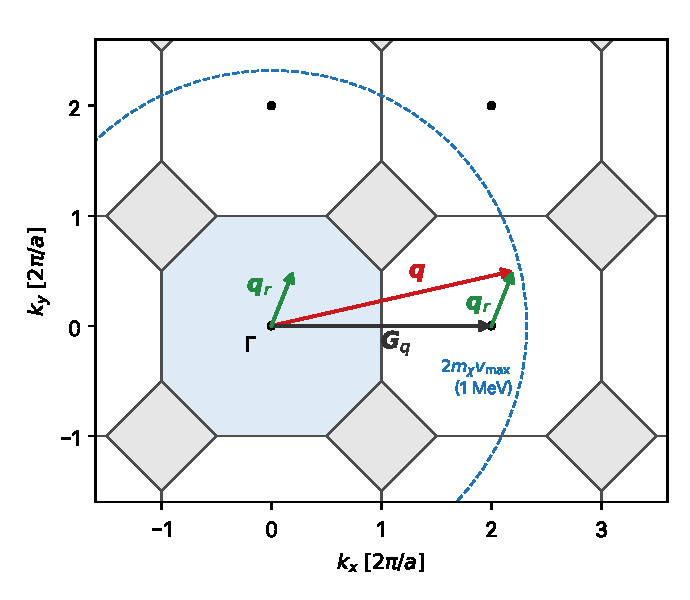
\includegraphics[width=0.62\linewidth]{figures/ch03/fig3_3.pdf}
  \caption{A momentum transfer reduced to the first Brillouin zone, in the plane $k_z = 0$ of the fcc reciprocal lattice, with momenta in units of $2\pi/a$ (\SI{2.28}{keV} for silicon). Dots: the reciprocal-lattice vectors in this plane, $(2\pi/a)(2m,2n,0)$. Octagons: the cuts of their Brillouin zones by the plane; the first zone is shaded blue. The grey squares belong to zones centered on reciprocal-lattice vectors $(2\pi/a)(h,k,\pm1)$ with $h, k$ odd, which lie outside the plane. The momentum transfer $\vect{q} = (2\pi/a)(2.2, 0.5, 0)$, of length \SI{5.15}{keV}, is the sum of the reciprocal-lattice vector $\vect{G}_q = (2\pi/a)(2,0,0)$ nearest to it and of $\vect{q}_r = (2\pi/a)(0.2, 0.5, 0)$, of length \SI{1.23}{keV}, drawn both at $\vect{G}_q$ and at the origin. Dashed circle: the maximum momentum transfer $2\mchi v_{\mathrm{max}} = \SI{5.30}{keV}$ of dark matter of mass \SI{1}{MeV}, with $v_{\mathrm{max}} = \SI{794.5}{km.s^{-1}}$.}
  \label{fig:3-umklapp}
\end{figure}

The momentum transfer itself is never reduced to the first zone. The dark matter loses $\vect{q}$, not $\vect{q}_r$, and its kinematics, $\vmin$ and the dark-matter form factor $\FDM(q)$ (\cref{sec:1.3,sec:1.4}) depend on $|\vect{q}|$. The target does not treat $\vect{q}$ and $\vect{q}_r$ alike either. Both change the crystal momentum by the same amount. However, the plane wave $\ee^{\ii\vect{q}\cdot\vect{r}}$ varies on the scale $2\pi/|\vect{q}|$ and resolves the electron density inside the cell on that scale. At large $|\vect{G}_q|$ it probes the region near the nuclei, where the core electrons and the steep part of the valence wavefunctions sit (\cref{sec:3.5}). The response of the crystal is therefore a function of $\vect{q}_r$ and $\vect{G}_q$ separately, not of $\vect{q}_r$ alone, and the book keeps both (\cref{app:A.3}).

\begin{workedexample}{Momentum transfers against the zone of silicon}\label{we:3-scales}
With $\hbar c = \SI{1973.27}{eV.\angstrom}$ and $a = \SI{5.431}{\angstrom}$,
\begin{equation*}
  \frac{2\pi}{a} = \frac{2\pi \times \SI{1973.27}{eV.\angstrom}}{\SI{5.431}{\angstrom}} = \SI{2283}{eV} = \SI{2.28}{keV} .
\end{equation*}
The shortest reciprocal-lattice vectors are $|\vect{G}_{111}| = \SI{3.95}{keV}$ and $|\vect{G}_{200}| = \SI{4.57}{keV}$. An electronic excitation across the low-temperature gap, $\Eg = \SI{1.17}{eV}$ (\cref{sec:3.3}), needs $q \ge \Eg/v_{\mathrm{max}} = \SI{1.17}{eV}/(2.650\times10^{-3}) = \SI{0.44}{keV}$, or $0.19\,(2\pi/a)$, deep inside the zone. The largest momentum transfer that can still deposit $\Eg$ follows from \cref{eq:1.3-region}, $q = \mchi v_{\mathrm{max}}[1 + (1 - 2\Eg/\mchi v_{\mathrm{max}}^2)^{1/2}]$. It is \SI{4.81}{keV} $= 2.11\,(2\pi/a)$ for $\mchi = \SI{1}{MeV}$, \SI{52.6}{keV} $= 23.0\,(2\pi/a)$ for \SI{10}{MeV} and \SI{530}{keV} $= 232\,(2\pi/a)$ for \SI{100}{MeV}. The lower end of the range is \SI{0.49}{keV} at \SI{1}{MeV} and tends to $\Eg/v_{\mathrm{max}} = \SI{0.44}{keV}$ for heavier particles, hardly depending on the mass; the upper end grows in proportion to $\mchi$.

Already at \SI{1}{MeV} the range extends past the eight $\vect{G}_{111}$ and the six $\vect{G}_{200}$, and the typical momentum of a valence electron, $q_0 = \SI{3.73}{keV} = 1.63\,(2\pi/a)$, lies outside the zone. A ball of radius $q$ contains about $(4\pi/3)q^3/[4(2\pi/a)^3]$ reciprocal-lattice vectors, one per zone volume. For the maximum momentum transfer $2\mchi v_{\mathrm{max}}$ this is $\num{1.3e4}$ at \SI{10}{MeV}, which a direct count confirms, and $\num{1.3e7}$ at \SI{100}{MeV}. Above about a MeV, most of the kinematically allowed momentum transfers have $\vect{G}_q \neq 0$, and a calculation of the rate must carry the response out to reciprocal-lattice vectors whose number grows as $\mchi^3$ (\cref{sec:3.5,app:E.7}).
\end{workedexample}

\subsection{The basis structure factor}

The positions of the atoms within the cell enter every Fourier component of a lattice-periodic quantity. Consider a function built from one term per atom, $f(\vect{r}) = \sum_{\vect{R}}\sum_\kappa v_\kappa(\vect{r} - \vect{R} - \vect{\tau}_\kappa)$, such as the potential of the clamped nuclei or a superposition of atomic charge densities. Its components, \cref{eq:A.3-periodic}, are
\begin{equation*}
  f_{\vect{G}} = \frac{1}{\Omega}\int_\Omega\dd^3r\;\ee^{\ii\vect{G}\cdot\vect{r}}\sum_{\vect{R}}\sum_\kappa v_\kappa(\vect{r} - \vect{R} - \vect{\tau}_\kappa)
  = \frac{1}{\Omega}\sum_\kappa\int\dd^3r\;\ee^{\ii\vect{G}\cdot\vect{r}}\,v_\kappa(\vect{r} - \vect{\tau}_\kappa) .
\end{equation*}
In the second step, the translate of the cell by $-\vect{R}$ was used for each term; since $\ee^{\ii\vect{G}\cdot\vect{R}} = 1$, the phase is unchanged, and the cells together fill all of space. Shifting $\vect{r}$ by $\vect{\tau}_\kappa$ then gives
\begin{equation}
  f_{\vect{G}} = \frac{1}{\Omega}\sum_\kappa\ee^{\ii\vect{G}\cdot\vect{\tau}_\kappa}\,\tilde v_\kappa(\vect{G}),
  \qquad \tilde v_\kappa(\vect{G}) = \int\dd^3x\;\ee^{\ii\vect{G}\cdot\vect{x}}\,v_\kappa(\vect{x}) .
  \label{eq:3.1-fG}
\end{equation}
Each atom contributes the transform of its own term at $\vect{G}$, with a phase set by its position in the cell. When all atoms of the basis are of one element, $\tilde v_\kappa = \tilde v$, the positions factor out into the \emph{basis structure factor}
\begin{equation}
  S^{\mathrm{bas}}(\vect{G}) = \sum_\kappa\ee^{\ii\vect{G}\cdot\vect{\tau}_\kappa},
  \label{eq:3.1-Sbas}
\end{equation}
and $f_{\vect{G}} = S^{\mathrm{bas}}(\vect{G})\,\tilde v(\vect{G})/\Omega$. A zero of $S^{\mathrm{bas}}$ is an \emph{extinction}: the component vanishes at that reciprocal-lattice vector, whatever the atomic term, because the contributions of the atoms in the cell cancel.

The nuclei of \cref{sec:2.3} are the simplest case. Their density for site $\kappa$, $n_\kappa(\vect{k}) = \sum_{\vect{R}}\ee^{\ii\vect{k}\cdot(\vect{R} + \vect{\tau}_\kappa)}$, becomes with \cref{eq:3.1-latticesum}
\begin{equation*}
  \sum_\kappa Z_\kappa\,n_\kappa(\vect{k}) = N\sum_{\vect{G}}\delta_{\vect{k},\vect{G}}\sum_\kappa Z_\kappa\,\ee^{\ii\vect{G}\cdot\vect{\tau}_\kappa} ,
\end{equation*}
nonzero only at reciprocal-lattice vectors, as \cref{sec:2.3} anticipated. The electron--nucleus potential of \cref{eq:2.3-HC} then has the components of \cref{eq:3.1-fG} with $\tilde v_\kappa(\vect{G}) = -Z_\kappa v_{\mathrm{C}}(|\vect{G}|)$. The same expression describes dark matter that couples to the clamped nuclei: it can transfer only a reciprocal-lattice vector, elastically, with no energy deposited. This is the coherent, Bragg-like part of the response mentioned in \cref{sec:2.2}, and a static lattice has no other nuclear response. Energy reaches the nuclei once they are allowed to move (\cref{chap:5}).

\begin{workedexample}{The diamond structure factor and the absent (200) reflection}\label{we:3-diamond}
For $\vect{G} = (2\pi/a)(h,k,l)$ and the basis of \cref{eq:3.1-basis}, $\vect{G}\cdot\vect{\tau}_2 = (\pi/2)(h + k + l)$, and \cref{eq:3.1-Sbas} gives
\begin{equation*}
  S^{\mathrm{bas}}(\vect{G}_{hkl}) = 1 + \ee^{\ii\pi(h + k + l)/2} .
\end{equation*}
For $h, k, l$ all odd, $h + k + l$ is odd and $S^{\mathrm{bas}} = 1 \pm \ii$, with $|S^{\mathrm{bas}}|^2 = 2$; for (111), $h + k + l = 3$ and $S^{\mathrm{bas}} = 1 - \ii$. For $h, k, l$ all even, $h + k + l$ is even, and two cases arise. If $h + k + l$ is a multiple of four, as for (220) and (400), the two atoms add in phase, $S^{\mathrm{bas}} = 2$ and $|S^{\mathrm{bas}}|^2 = 4$. If $h + k + l = 4n + 2$, as for (200) and (222), $S^{\mathrm{bas}} = 1 + \ee^{\ii\pi} = 0$. The plane wave at $\vect{G}_{200}$ has its crests on the atoms at $\vect{\tau}_1$ and its troughs on those at $\vect{\tau}_2$, a quarter cube diagonal away, and the two contributions cancel.

The (200) and (222) reflections of silicon are therefore absent in X-ray diffraction from spherical atoms, although $\vect{G}_{200}$ and $\vect{G}_{222}$ are reciprocal-lattice vectors of its fcc lattice and $\vect{G}_{200}$ is the second-shortest. The same cancellation removes these components from any part of the crystal potential that is a sum of identical spherical atomic terms. The (222) component returns through the part of the potential that is not of this form, such as the charge that piles up in the bonds (\cref{sec:3.4}), and is observed as a weak X-ray reflection. The (200) component does not. The diamond structure is mapped onto itself by \emph{glides}, each a reflection in a plane parallel to a cube face followed by a translation by a quarter of a face diagonal within that plane. The glides force it to vanish for every function with the symmetry of the crystal (\cref{app:C.17}). In zincblende GaAs the two sites hold different nuclei, $Z_\kappa = 31$ (gallium) and 33 (arsenic), and the nuclear factor $\sum_\kappa Z_\kappa\ee^{\ii\vect{G}\cdot\vect{\tau}_\kappa}$ equals $31 - 33 = -2$ at (200), against $31 + 33 = 64$ at (220). The (200) component is weak, smaller in square by a factor of $4/4096 \approx 10^{-3}$, but not zero, and it is what distinguishes the zincblende structure from diamond in diffraction.
\end{workedexample}

Extinctions also explain why the fcc reciprocal lattice lacks the vectors $(2\pi/a)(h,k,l)$ of mixed parity. The fcc lattice can also be described as a simple cubic lattice of side $a$ with a basis of four points, at a corner and the three adjacent face centers. Its reciprocal lattice is then simple cubic, $(2\pi/a)(h,k,l)$ with any integers, and the structure factor of the four points is $1 + \ee^{\ii\pi(h + k)} + \ee^{\ii\pi(k + l)} + \ee^{\ii\pi(l + h)}$, which is 4 when $h, k, l$ have one parity and 0 otherwise. A basis structure factor is the price of using a cell larger than the primitive one, and its zeros remove exactly the vectors that the smaller cell does not have.

The electrons move in the periodic potential whose components \cref{eq:3.1-fG} describes. \Cref{sec:3.2} shows that their states are labeled by a crystal momentum in the zone and a band index, and computes the matrix element of $\ee^{\ii\vect{q}\cdot\vect{r}}$ between them, with the Umklapp vector kept in the plane wave.
